\documentclass{article}
% if you need to pass options to natbib, use, e.g.:
%     \PassOptionsToPackage{numbers, compress}{natbib}
% before loading neurips_2020

% ready for submission
% \usepackage{neurips_2020}

% to compile a preprint version, e.g., for submission to arXiv, add add the
% [preprint] option:
%     \usepackage[preprint]{neurips_2020}

% to compile a camera-ready version, add the [final] option, e.g.:
%     \usepackage[final]{neurips_2020}

% to avoid loading the natbib package, add option nonatbib:
\PassOptionsToPackage{numbers, compress}{natbib}
\usepackage{neurips_2020}
\bibliographystyle{plainnat}
% \usepackage{biblatex}
% \addbibresource{references.bib}

\usepackage[utf8]{inputenc} % allow utf-8 input
\usepackage[T1]{fontenc}    % use 8-bit T1 fonts
\usepackage{hyperref}       % hyperlinks
\usepackage{url}            % simple URL typesetting
\usepackage{booktabs}       % professional-quality tables
\usepackage{amsfonts}       % blackboard math symbols
\usepackage{nicefrac}       % compact symbols for 1/2, etc.
\usepackage{microtype}      % microtypography
\usepackage[ruled, vlined]{algorithm2e}
\usepackage{graphicx}
\usepackage{multirow}
\graphicspath{{figures/}}

\title{DeepMDRP: A Multi-task CNN based approach towards resistance prediction in MTB isolates}

% The \author macro works with any number of authors. There are two commands
% used to separate the names and addresses of multiple authors: \And and \AND.
%
% Using \And between authors leaves it to LaTeX to determine where to break the
% lines. Using \AND forces a line break at that point. So, if LaTeX puts 3 of 4
% authors names on the first line, and the last on the second line, try using
% \AND instead of \And before the third author name.

\author{%
  David S.~Hippocampus\thanks{Use footnote for providing further information
    about author (webpage, alternative address)---\emph{not} for acknowledging
    funding agencies.} \\
  Department of Computer Science\\
  Cranberry-Lemon University\\
  Pittsburgh, PA 15213 \\
  \texttt{hippo@cs.cranberry-lemon.edu} \\
  % examples of more authors
  % \And
  % Coauthor \\
  % Affiliation \\
  % Address \\
  % \texttt{email} \\
  % \AND
  % Coauthor \\
  % Affiliation \\
  % Address \\
  % \texttt{email} \\
  % \And
  % Coauthor \\
  % Affiliation \\
  % Address \\
  % \texttt{email} \\
  % \And
  % Coauthor \\
  % Affiliation \\
  % Address \\
  % \texttt{email} \\
}

\begin{document}

\maketitle

\begin{abstract}
  In this report we explore the problem of predicting phenotypic susceptibility of MTB isolates
towards 10 drugs including 4 first line drugs and 4 second line drugs. We experiment with a number
of statistical models for predicting MTB resistance towards different drugs and propose a Deep Convolutioal
Neural Network that achieves state of the art results in predicting MTB resistance in all the first and
second line drugs while achieving competitive performance on other drugs. We also give a detailed report
of several approaches that were critical in the performance of our method while also giving a detailed account
of approaches that did not perform as well, hoping that it would be helpful to the research community. The source
code for our approach is publicly available at \emph{https://github.com/kpandey008/drug-resistance-prediction}
\end{abstract}

\section{Introduction}

Tuberculosis is one of the top 10 leading causes of mortality worldwide and the leading cause
of death from a single infectious agent, caused by the bacillus \emph{Mycobacterium Tuberculosis (MTB)}
\cite{10665-329368}. To make the situation even more difficult to tackle, there has been a significant rise of
drug-resistant bacterial strains due to the increasing use of antibacterial drugs. Moroever, the phenotypic
drug susceptibility test (DST) that determines which drugs are effective towards particular TB infections
is slow and costly.

\setlength{\parindent}{2ex}
Recently, methods involving Whole Genome Sequencing(WGS) of MTB have emerged as a faster alternative for
identifying drug-resistant TB \cite{article}. A number of Single Nucleotide Polymorphisms (SNP) have been identified that are associated
with drug resistance found in MTB isolates. However, the interactions between different SNP's associated 
with drug resistance in MTB isolates is complex and cannot be modeled efficiently using rule-based
methods that incorporate significant domain knowledge when predicting MTB resistance towards a particular drug.
More recently, there has been a surge in using Machine learning(ML) methods for tackling this problem as a predictive
modeling problem where the SNP's for MTB isolates are used as features and the model needs to predict if the
isolate is resistant to a particular drug. \cite{10.1093/bioinformatics/btx801} provide a comparison between several classical ML methods like
Logistic Regression, Random Forests (RF) and Support Vector Machines (SVM) to predict MTB resistance to 11 assayed drugs
including 4 first line drugs (Rifampicin (RIF), Isoniazid (INH), Ethambutol (EMB), Pyrazinamide (PZA)) and
6 second line drugs (Streptomycin (STR), Capreomycin (CAP), Ciprofloxacin (CIP), Kanamycin (KAN), Moxifloxacin(MOXI),
Amikacin (AMK), Ofloxacin (OFX)). \cite{CHEN2019356} pose the resistance prediction problem as a multi-task learning problem where
they use a Deep neural network (WDNN) to predict resistance of MTB isolates for all the 11 drugs using a single
neural network. \cite{10.1093/bioinformatics/btz067} pretrain a Deep de-noising autoencoder to learn latent representations over the binary SNP features
and use the resulting autoencoder in composition with a classifier to predict MTB resistance towards the first-line drugs.\\

In this report, we propose DeepMDRP, a multi-task Deep Convolutional Neural Network (CNN) for predicting resistance of MTB isolates
towards 10 drugs (excluding CIP). We provide several justifications for our model choice and show that our
approach outperforms existing approaches when predicting MTB resistance in most first and second line drugs. The rest of
the report is organized as follows:

\section{Deep MTB Drug Resistance Predictor (DeepMDRP)}
\label{headings}

In this section we present an overview of our network. As shown in Figure \ref{fig:architecture} our network takes a batch of
feature vectors as an input of the form $B \times 1 \times d$ where B is the batch size and d is the dimension of the feature
vector. Here, each feature vector is representative of a single MTB isolate and each dimension of the feature vector
is a binary value which represents whether a mutation occurs in that isolate (1) or not (0).
This feature vector is passed through a Deep CNN which outputs a prediction vector
of size equal to the number of drugs considered in the analysis. Therefore, the output prediction vector
would be a 11 dimensional vector that outputs the probabililty estimates of resistance of the MTB isolate
of each drug in the order: $\{RIF, INH, PZA, EMB, STR, CIP, CAP, AMK, MOXI, OFLX, KAN\}$

\subsection{Network Architecture}
\begin{figure}[t]
  \centering
  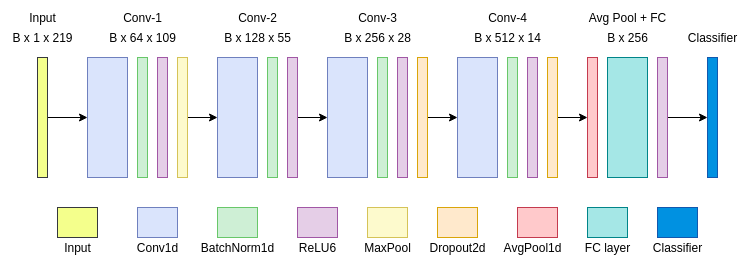
\includegraphics[scale=0.5]{architecture.png}
  \caption{Network Architecture. The dimensions above each block represent the shape of the output of that module
  . The output of the Conv module is of the form (B x C x d) where B is the batch size, C is the number of channels,
  and d is the feature length. The output of the FC module is (B x d).}
  \label{fig:architecture}
\end{figure}

The network architecture for the Deep CNN is shown in Figure \ref{fig:architecture}. It takes a $B \times d$ 
dimensional input where B
is the batch size and d is a 219 dimensional feature vector. The CNN network consists of four 1-d convolutional blocks
followed by a fully connected block and a classifier layer. The input B x 219 dimensional feature vector is 
first reshaped into a B x 1 x 219 dimensional
tensor which is then input to the network. As shown in Figure \ref{fig:architecture}, we use BatchNorm1d \cite{43442}
and Dropout2d \cite{DBLP:journals/corr/TompsonGJLB14} modules
to regularize training. We use the ReLU6 activation as opposed to ReLU as it gave better empirical performance
during evaluation. We choose CNN's as a prediction model for this problem in contrast to other ML models 
for the following reasons:

\begin{itemize}
    \item CNN's can operate on sequences of varying length as they are independent of the input size. 
    This allows us to
    experiment with transfer learning approaches which have been successfully applied to several problems in 
    vision and
    NLP.
    Note that this is not possible with a simple deep MLP which is dependent of the size of the input features.
    \item CNN's promote parameter sharing which has two advantages. It allows us to detect recurring patterns in
    sequences and allows for a reduction in the parameter count. This further enables us to build deeper models that
    can capture complex patterns between mutations.
    \item CNN's build more abstract features at each layer and thus are able to learn more complex patterns. 
    We hypothesize
    that this behavior might be important to model complex co-occuring patterns between different mutations. 
\end{itemize}

\subsection{Training and Testing}

The training procedure for our network is described in Algorithm \ref{algo:train}. One
important aspect of our training algorithm is the use of Mixup \cite{DBLP:journals/corr/abs-1710-09412} data augmentation. As we discuss in the
experimental details, Mixup leads to an improved overall performance of the network and prevents the
network from overfitting. We choose the masked binary cross entropy loss as the loss criterion
as the dataset contains -1 labels for some drugs which needs to be masked during training.
We use the Adam \cite{kingma2017adam} optimizer for weight update and the gradient updates are made through backpropagating through
the network. The training Hyperparameters are discussed in section \ref{section:hyper}\\
The testing procedure is simple as it involves only a single forward pass of the test sample through
the trained network.

\begin{algorithm}[H]
    \SetKwInOut{Input}{Input}\SetKwInOut{Output}{Output}
    \SetAlgoLined
     \Input{Training set $D$, Initialized model: $M$, Hyperparameters: $\{num\_epochs, \alpha, \eta, \beta_1, \beta_2\}$}
     \Output{Trained model $M$}
     \BlankLine
     \For{$i \leftarrow 1$ \KwTo $num\_epochs$}{
     \For{$X_{batch}, Y_{batch}\in D$}{
        $mixup \sim \mathcal{U}(0,1)$\;
        \eIf{$mixup > 0.5$}{
            $\lambda \sim Beta(\alpha, \alpha) $\;
            $\hat{X} = permute(X_{batch})$\;
            $\hat{Y} = permute(Y_{batch})$\;
            $X_{mixup} = \lambda X_{batch} + (1 - \lambda)\hat{X}$\;
            $Y_{pred} = \sigma(M(X_{mixup}))$\;
            $loss = \lambda * binary\_cross\_entropy(Y_{pred}, Y_{batch}) + (1 - \lambda) * binary\_cross\_entropy(Y_{pred}, \hat{Y})$
        }{
            $Y_{pred} = \sigma(M(X_{batch}))$\;
            $loss = binary\_cross\_entropy(Y_{pred}, Y_{batch})$
        }
        $w \leftarrow Adam(\eta, \beta_1. \beta_2)$
     }
     }
    \caption{Algorithm for training DeepMDRP}
    \label{algo:train}
\end{algorithm}

\section{Experimental Details}

\subsection{Dataset}
The dataset used for training consists of 3393 samples with 222 features. In the provided dataset some features
have missing values. More specifically, the features $SNP\_CN\_2714366\_C967A\_V323L\_eis$,
$SNP\_I\_2713795\_C329T\_inter\_Rv2415c\_eis$, $SNP\_I\_2713872\_C252A\_inter\_Rv2415c\_eis$ have missing values.
We remove these features from the dataset resulting in 219 binary features (Each feature representing
a mutation). The targets provided in the dataset also have missing values which we mask during training. We use
a validation set of 792 samples taken from \cite{CHEN2019356} as the authors in this paper use the same feature set as ours
to evaluate their model performance.

\subsection{Implementation Details}
\label{section:hyper}

\textbf{Model}: The model architecture as shown in Figure \ref{fig:architecture} is a multi-task architecture that 
consists of 4 Conv1d layers containing
{64, 128, 256, 512} filters respectively. Each conv layer is followed by a BatchNorm1d layer and a ReLU6
activation. The first conv layer also uses a MaxPool1d layer after applying the ReLU6 activation. In the
last two Conv blocks we use a Dropout2d module with a drop probability of 0.3. The output of the last conv
block is fed into a AveragePooling layer followed by a flatten operation. The resulting output is then
fed into a fully-connected layer -> ReLU6 -> BN unit. The final output is then fed into a classifier which
makes predictions for individual drugs.

\textbf{Training}: We use PyTorch \cite{paszke2019pytorch} for developing the neural net
framework developmnent and training. We train our DeepCNN predictor for 100 epochs with a batch size of 32
using the Adam optimizer. The mixup parameter $\alpha$ is set to 2.0. The initial
learning rate is set to 0.001 and weight decay to 0.0001. We adjust the learning rate using the Cosine Annealing
scheduler with warm restarts \cite{loshchilov2017sgdr} ($T_0 = 10$ and $t_{mul}=2$). For computing loss, we use a custom masked
Binary cross entropy (BCE) loss without any weight balancing. We train the entire system on the Google Colab
platform.

\subsection{Ablation Studies}
For the results in this section, we report the AUC scores on our validation set of 792 isolates.
We evaluate the model performance on the best performing checkpoint for each method and do
not perform any ensembling for any of the methods. We do not change the training settings for these
experiments unless mentioned otherwise.

\subsubsection{Choice of Models}
Apart from using a Deep-CNN as a model for our experiments we also tried a number of other approaches as follows:
\begin{itemize}
  \item We created a deep-MLP containing three fc blocks (Linear -> BatchNorm1d -> ReLU 
  Dropout(0.5))
  This architecture is similar to the WDNN used in \cite{CHEN2019356} so we denote this network architecture as WDNN. We
  experiment with two variants of WDNN. One with all hidden layers of dimension 256 and one with 512. We refer
  to these models as \emph{WDNN-256} and \emph{WDNN-512} respectively.
  \item We also experimented with self-attention based models \cite{vaswani2017attention}. The primary intuition behind using these models
  was to model correlations between mutations as these models have recently been shown to be extremely
  efficient in modeling long term dependencies in sequences in several NLP and computer vision tasks.
  We implement
  a MultiHead attention module and use this layer at the end of the conv blocks in the DeepCNN. We denote
  this model as \emph{DeepCNN-MH}.
  \item We also experimented with different layer normalization methods. More specifically we tried
  using a Weight standardization \cite{qiao2020microbatch} + GroupNorm \cite{wu2018group} (WS + GN) in combination with the DeepCNN. The intuition behind
  this choice is based on the fact that WS + GN has been shown to stabilize gradients during training
  which might improve performance. We denote this model by DeepCNN (WS + GN)
  \item Another variant that we tried is based on using Squeeze and Excitation \cite{hu2019squeezeandexcitation} (SE) units in combination
  with the DeepCNN architecture. We denote this model by DeepCNN-SE.
  \item Lastly, we tried involved pre-processing the input features using dimensionality reduction
  methods and then using the pre-processed features as inputs to our model.
  We specifically tried two such methods: kernel-PCA and NMF and denote these methods as \emph{DeepCNN-kPCA} and 
  \emph{DeepCNN-NMF} respectively. The dimension of the features using these methods was reduced to 100.

\end{itemize}
\begin{table}[t]
  \centering
  \caption{Model performance comparison on the Multitask prediction task.}
  \begin{tabular}{lllll}
      \toprule
      \multirow{1}{*}[0em]{Models} & Avg. AUC\\
      % \addlinespace[1pt]
      \midrule
      DeepCNN & 94.5 \\
      WDNN-256 & 94.5 \\
      WDNN-512 & \textbf{94.7} \\
      DeepCNN (WS + GN) & 94.4 \\
      DeepCNN-SE & 94.4 \\
      DeepCNN-MH (8 heads) & 93.7 \\
      DeepCNN-NMF & 81.6 \\
      DeepCNN-kPCA & 66.8 \\
      \bottomrule
  \end{tabular}
  \label{table:model_tb}
\end{table}
The performance of this model on multi-task drug resistance prediction is shown in Table \ref{table:model_tb}
As can be observed, any kind of pre-processing on the data severely affects the performance of the model.
Out of all the models, WDNN-512 performs the best with a average AUC score of 94.7. DeepCNN and WDNN-256
perform similiarly on the prediction task. It was surprising to see DeepCNN with multi-head attention not
performing as expected. We hypothesize that this architecture needs more experimentation. Also MultiHead
attention performs really well on a large amount of data, which is not the case here. This could be another
reason for the architecture achieving lesser AUC scores.


\subsubsection{Choice of Loss function}
Apart from using the Masked Binary Cross Entropy Loss (BCE), we also experimented with Masked versions of Mean Squared Loss
(MSE), L1 Loss (MAE), and Online Hard Example Mining (OHEM)\cite{shrivastava2016training} version of BCE. OHEM selects
samples from the training batch for which the computed loss is the highest and backpropagates
through only these hard examples. We used a value of 15 hard examples for each drug. The model used for this experiment
was the Multitask Deep-CNN predictor. The results for these variants are given in Table \ref{table:loss_tb}.
As evident from the results, masked BCE performs the best among all the variants so we use it for our final model.
\begin{table}[t]
  \begin{minipage}{0.5\linewidth}
  \centering
  \caption{Model performance comparison for different loss functions.}
  \begin{tabular}{lllll}
      \toprule
      \multirow{1}{*}[0em]{Masked Loss} & Avg. AUC\\
      % \addlinespace[1pt]
      \midrule
      BCE & \textbf{94.5} \\
      MSE & 93.7 \\
      MAE & 93.7 \\
      OHEM-BCE & 93.8 \\
      \bottomrule
  \end{tabular}
  \label{table:loss_tb}
\end{minipage}
\begin{minipage}{0.5\linewidth}
  \centering
  \caption{Effect of weight balancing methods}
  \begin{tabular}{lllll}
      \toprule
      \multirow{1}{*}[0em]{Method} & Avg. AUC\\
      % \addlinespace[1pt]
      \midrule
      Unweighted & \textbf{94.5} \\
      Inverse & 93.8 \\
      Pos-Neg & 93.9 \\
      Median & 93.7 \\
      \bottomrule
  \end{tabular}
  \label{table:weight_balance}
\end{minipage}
\end{table}


\subsubsection{Dataset imbalance}
The training data used for our experiments suffers from the common problem of class imbalance. We hypothesized
that some form of weight balancing would be needed during training. Due to this reason, we experimented with
three types of weight balancing schemes during training.
\begin{itemize}
  \item \emph{Inverse Frequency Balancing} : This computes the normalized inverse class frequencies for each drug.
  \item \emph{Median frequency balancing} which computes the inter-class median 
  frequency and computes class weights by $median / class\_freq$ for each drug. In this way minority classes have weights
  greater than 1 and majority classes have weights < 1.
  \item Lastly, we also experimented by measuring the ratio of
  the frequencies of the positive and the negative samples and using those weights for the positive class during
  training for each drug. This is equivalent to subsampling methods in which we can either oversample the minority
  class or undersample the majority class.
\end{itemize}
  However, none of these schemes worked better than the unweighted version of our classifier.
The results are shown in Table \ref{table:weight_balance}.

\subsubsection{Choice of Optimizer}
Apart from the Adam optimizer, we experimented with Stochastic Gradient Descent (SGD), RMSProp and AdamW \cite{loshchilov2019decoupled} 
optimizers. The learning rate for all the optimizers was set to 0.001. We found
similiar performance for different kinds of optimizers. However, SGD took longer to
converge so we selected Adam as the final choice for the model.

\subsubsection{Choice of Learning Rate Scheduler}
We use the Cosine Annealing learning rate scheduler with warm restarts \cite{loshchilov2017sgdr}.
We also experimented with a Poly learning rate policy and a Step scheduler.

\subsubsection{Regularization strategies}
Since, our training dataset size is relatively small (only 3393) samples, we experiment with a number of
regularization strategies. Apart from Mixup and Dropout2d, we tried Dropout \cite{JMLR:v15:srivastava14a}, Label Smoothing \cite{pereyra2017regularizing} and adding noise
to the input data. However, Mixup plays a very important role in improving the performance of the models
as demonstrated in Table \ref{table:mixup}. It is worth noting that the DeepCNN model benefits the
most from Mixup.

\subsubsection{Impact of transfer learning}
\begin{table}[t]
  \begin{minipage}{0.5\linewidth}
  \centering
  \caption{Finetuning vs Train-from-scratch}
  \begin{tabular}{lllll}
      \toprule
      \multirow{1}{*}[0em]{Drug} & With Fine-tuning & W/o fine-tuning\\
      % \addlinespace[1pt]
      \midrule
      RIF & 98.6 & \textbf{98.7} \\
      INH & \textbf{97.4} & 97.1 \\
      PZA & \textbf{90.6} & 89.3 \\
      EMB & \textbf{92.6} & 91.7 \\
      \bottomrule
  \end{tabular}
  \label{table:finetune}
\end{minipage}
\begin{minipage}{0.5\linewidth}
  \centering
  \caption{Effect of Mixup}
  \begin{tabular}{lllll}
      \toprule
      \multirow{1}{*}[0em]{Model} & With Mixup & W/o Mixup\\
      % \addlinespace[1pt]
      \midrule
      DeepCNN & 94.5 & 93.9 \\
      WDNN256 & 94.5 & 94.3 \\
      WDNN512 & 94.7 & 94.2 \\
      \bottomrule
  \end{tabular}
  \label{table:mixup}
\end{minipage}
\end{table}
As pointed in section 2, using a Deep-CNN can enable strategies like Transfer learning which can be very
efficient when using less amount of labeled data. Transfer learning involves fine-tuning a classifier
which has been pre-trained on a similiar source task so that a target task with less data can benefit
from the training of the source task trained with a large amount of data. For pre-training, we train our
Deep-CNN classifier on the DeepAMR \cite{10.1093/bioinformatics/btz067} dataset which consists of 
8390 samples with 5824 mutations for
predicing MTB resistance to the four first line drugs. We then fine-tune our classifier on our target
dataset to predict MTB resistance towards the assayed drugs. The results are shown in Table \ref{table:finetune}
As evident from the results, transfer learning certainly improves the performance of INH, EMB and PZA as
compared to its train-from-scratch DeepCNN counterpart.



\section{Final Performance}
\begin{table}[t]
  \begin{minipage}{0.5\linewidth}
  \centering
  \caption{WDNN[] vs DeepCNN performance}
  \begin{tabular}{lllll}
      \toprule
      \multirow{1}{*}[0em]{Drug} & WDNN & DeepCNN\\
      % \addlinespace[1pt]
      \midrule
      RIF & 98.2 & \textbf{98.4}\\
      INH & 95.9 & \textbf{97.2} \\
      PZA & 88.3 & \textbf{89.0} \\
      EMB & \textbf{92.2} & 91.6 \\
      STR & \textbf{94.2} & 93.8\\
      CAP & \textbf{80.8} & 77.5 \\
      AMK & 95.0 & \textbf{97.7} \\
      MOXI & 90.2 & \textbf{95.6} \\
      OFLX & 86.6 & \textbf{86.9}\\
      KAN & 87.9 & \textbf{89.6} \\
      \bottomrule
  \end{tabular}
  \label{table:compare_sota}
\end{minipage}
\begin{minipage}{0.5\linewidth}
  \centering
  \caption{Kaggle Leaderboard scores}
  \begin{tabular}{lllll}
      \toprule
      \multirow{1}{*}[0em]{Drug} & Avg AUC\\
      % \addlinespace[1pt]
      \midrule
      RIF & 98.95 \\
      INH & 97.99 \\
      PZA & 92.50 \\
      EMB & 94.47 \\
      STR & 96.18 \\
      CAP & 87.55 \\
      AMK & 98.05  \\
      MOXI & 98.08  \\
      OFLX & 89.94 \\
      KAN & 93.21  \\
      \bottomrule
  \end{tabular}
  \label{table:kaggle_results}
\end{minipage}
\end{table}
In this section we compare the results of our multitask DeepCNN based approach with WDNN as specified in \cite{CHEN2019356} as
this is most relevant to our work. We use the same validation set 
which is used by \cite{CHEN2019356} in their evaluation. The results are shown in Table \ref{table:compare_sota}. As evident
from the results, our multi-task method beats the state of the art method performance on the majority 
of the drugs. We also submitted our evaluations to the Kaggle leaderboard as a part of the ongoing
competition. The results are shown in Table \ref{table:kaggle_results}. It is worth
noting that the results submitted to the Kaggle competitions were submitted using multiple
variants of WDNN256, WDNN512 and DeepCNN.

\section{Conclusion and Future Work}
In this report we present a novel DeepCNN based method with mixup augmentation
 for predicting drug resistance in MTB isolates. We show that our method achieves
better performance compared to the state of the art model on multiple first and 
second line drugs. We also
present an overview of different model variants that we experimented with and a 
detailed ablation study covering several aspects of model development including
choice of loss functions, optimizers, learning rate schedulers and regularization strategies
. To conclude,
we see the following directions as direct extensions to our work.
\begin{itemize}
  \item More experimentation with multi-head attention based models for modeling correlations
  between mutations.
  \item Since our dataset contains a lot of unlabeled data for different drugs. It would
  be interesting to explore the application of semi-supervised learning methods in 
  the multi-label context.
  \item Another direction could be to explore model / checkpoint averaging methods
  as a way to make the model predictions more robust which we have not explored as a part
  of this work.
\end{itemize}

\section{Contributions}
Kushagra contributed to:
\begin{itemize}
  \item Conducting literature review in MTB drug resistance and semi-supervised
  learning methods.
  \item Developing and testing the core network architecture presented in this report
  \item Ablation Studies (choice of loss functions, model variants etc.)
  \item Report Development
\end{itemize} 

\bibliography{references}

\end{document}